
\section{Proofs for Blindness}
\subsection{Correctness of Blind-State Injection}
\label{appendix: correctness of blind-gate}
\begin{proof}[Proof of correctness of Protocol~\ref{protocol:blind-gate}]
    When both parties behave honestly, we here show that the output of the protocol is identical to the one of the Ideal Resource.
    \paragraph{State received by the Server}
    Below, we write the state held by the Server after receiving encrypted qubits from the Client, including the ancilla register. The Client samples $n$-bit strings, additional encryption bits on the $n+1$-th index, and simply writes the total $n+1$-bit encryption keys $\a, \r$.
    Taking into account that the ancillary state (in register $n+1$) is pre-rotated by $\theta$, the Server receives
    \begin{align}
        \rho_{in}
        &=
        \X^{\a}
        \Z^{\r}
        \circ
        \Z_{n+1}(\theta)
        [
            \rho\otimes \rho_\A
        ]
    \end{align}
    \paragraph{State Injection by the Server.}
    The Server starts by performing the Clifford circuit $\C$ on the first $n$ qubits, and applies $\F$ (CNOT followed by a SWAP) on the total system.
    \begin{align}
        \rho_{inj} &=
        \F
            \circ
            \C
            [
                \rho_{in}
            ]
    \end{align}

    \paragraph{Measurement and Rotation.}
    The Server then measures qubit $n+1$ in the computational basis. Assuming it yielded outcome $b$, the Client computes $b'$ as mentioned in the protocol, computes the appropriate angle and blinds it, and the Server receives $\delta_{b'}$. In total, from the Server's point of view we can write that the system is in the state $\Z^{\dagger}_n(\delta_{b'})[\rho_{inj}]$ on which we apply the projector $\ketbra b$ on the $n+1$-th qubit. However since the Client stores the output bit as $b'$, the total system is actually in the state
    \begin{align}
        \rho_{dec}
        &=
        \ketbra{b'}{b}_{n+1}
        \circ
        \Z_n^\dagger(\delta_{b'})
        \left[
            \rho_{inj}
            \right]
        \end{align}

        \paragraph{Commuting the encryption.}
        We now re-write the above state by commuting the encryption.
        In the first line, we simply expand the above expression. In the second line, we commute the Pauli encryption through the Clifford circuit $\C$, then $\F$, on $n+1$ qubits. Note that this gives the Pauli $\Enc{\a'}{\r'}$ that the Client computes as well, in the protocol. Also, the $\theta$ rotation acts on the $n+1$-th bit, so it commutes trivially through $\C$ (which acts on the $n$ first qubits only). Then, through $\F$ it commutes with the $\CNOT$ since it acts on qubit $n+1$ which is the controlled qubit, and after the $\SWAP$ it ends up on the $n$-th qubit.
        This results in
        \begin{align}
            \rho_{dec}
            &=
            \ketbra{b'}{b}_{n+1}
            \circ
            \Z_n^\dagger(\delta_{b'})
            \circ
            \F
            \circ
            \C
            \circ
            \X^{\a}
            \Z^{\r}
            \circ
            \Z_{n+1}(\theta)
        [
            \rho\otimes \rho_\Apattern
        ]
        \\
            &=
            \ketbra{b'}{b}_{n+1}
            \circ
            \Z_n^\dagger(\delta_{b'})
            \circ
            \X^{\a'}
            \Z^{\r'}
            \circ
            \Z_{n}(\theta)
            \circ
            \F
            \circ
            \C
        [
            \rho\otimes \rho_\Apattern
        ]
        \end{align}
        And now, we are interested in commuting the encryption through the $\delta$ rotation on the $n$-th qubit. In the first line we just use the fact that this rotation acts on the $n$-qubit only, so the encryption on the other qubits commute trivially. On the second line, we use the fact that $\Z$ commutes through $\Z$-rotation and $\X$ commute up to a sign flip of the angle, and in the third line we just combine the operators again to have a compact notation. Finally in the last three lines we use the fact that $\Z(\alpha)\circ \Z(\beta) = \Z(\alpha+\beta)$, and replaced $\delta$ by its definition, which cancels out the $(-1)^{a_n'}$ sign introduced by commuting the encryption.
        \begin{align}
            \Z_n^{\dagger}(\delta) \circ \X^{\a'}\Z^{\r'} \circ \Z_{n}(\theta)
            &=
            \left(\bigotimes_{i\neq n}\X^{a'_i}\Z^{r'_i}\right)
            \otimes
            \left(\Z^{\dagger}(\delta) \circ \X^{a_n'}\Z^{r_n'}\right)
            \circ \Z_{n}(\theta)
            \\
            &=
            \left(\bigotimes_{i\neq n}\X^{a'_i}\Z^{r'_i}\right)
            \otimes
            \left(
                \X^{a_n'}\Z^{r_n'}
                \circ
                \Z^{\dagger}((-1)^{a_n'}\delta)
            \right)
            \circ \Z_{n}(\theta)
            \\
            &=
            \Enc{\a'}{\r'}
            \circ
            \Z_n^{\dagger}((-1)^{a_n'}\delta)
            \circ \Z_{n}(\theta)
            \\
            &=
            \Enc{\a'}{\r'}
            \circ
            \Z_n^{\dagger}((-1)^{a'_n}\times(-1)^{a_n'}(\phi_{b'}+\theta)-\theta)
            \\
            &=
            \Enc{\a'}{\r'}
            \circ
            \Z_n^{\dagger}(\phi_{b'})
        \end{align}

        Altogether, we can thus write
        \begin{align}
            \rho_{dec}
            &=
            \ketbra{b'}{b}_{n+1}
            \circ
            \X^{\a'}
            \Z^{\r'}
            \circ
            \Z_n^\dagger(\phi_{b'})
            \circ
            \F
            \circ
            \C
        [
            \rho\otimes \rho_\Apattern
        ]\; .
        \end{align}
        The next re-writing step is to interpret the Client's decoding of the measurement outcome as a decryption of the quantum state before measurement. This can be done by changing variables for $b$, as $b\mapsto b\oplus a_{n+1}'$. The consequence is that $b'$ becomes $b$ and $\ketbra{b'}{b}$ becomes $\ketbra{b}{b'} = \ketbra{b} \circ \X^{a_{n+1}'}$: flipping the measurement outcome is equivalent to applying a Pauli $\X$ upon measurement in computational basis. Furthermore, for the sake of homogeneity, we note that we can write it as a full decryption $\Dec{a'_{n+1}}{r'_{n+1}}$ as $\ketbra{b} \circ \X^{a_{n+1}'} = \ketbra{b} \circ \Z^{r'_{n+1}}\X^{a_{n+1}'}$ since up to a global and irrelevant phase, $\bra b \Z^r = \bra b$. Thus, the state of the total system, before decryption by the Client, is
        \begin{align}
            \rho_{dec, b}
            &=
            \left(
            \ketbra{b}{b}
            \circ
                \Dec{a'_{n+1}}{r'_{n+1}}\right)_{n+1}
            \circ
            \Enc{\a'}{\r'}
            \circ
            \Z_n^\dagger(\phi_{b})
            \circ
            \F
            \circ
            \C
        [
            \rho\otimes \rho_\A
        ]
    \end{align}
    \paragraph{Client decryption.}
    Finally, the Client applies $\Dec{\tilde\a'}{\tilde\r'}$ defined as $\Dec{\a'}{\r'}$ if $\A\neq \Tlabel$, and $\X^{b}_n\circ\Dec{\a'}{\r'}$ if $\A=\Tlabel$. In both cases, the additional correction is Pauli and acts on the $n$-th qubit, so it commutes with $\ketbra b_{n+1}$.
    \begin{itemize}
        \item In the $\A\neq \Tlabel$ case, then it is straightforward that
        \begin{align}
            \rho_{out, b}
            &=
            \ketbra b_{n+1}
            \circ
            \underbrace{(\bigotimes_{i\leq n}\Dec{a'_i}{r'_i})
            \circ
            (\Dec{a'_{n+1}}{r'_{n+1}})_{n+1}}_{\Dec{\a'}{\r'}}
            \circ
            \Enc{\a'}{\r'}
            \circ
            \Z_n^\dagger(\phi_{b})
            \circ
            \F
            \circ
            \C
        [
            \rho\otimes \rho_\A
        ]
        \nonumber
        \\
        &=
            \ketbra b_{n+1}
            \circ
            \underbrace{\Dec{\a'}{\r'}
            \circ
            \Enc{\a'}{\r'}}_{\id_{n+1}}
            \circ
            \Z_n^\dagger(\phi_{b})
            \circ
            \F
            \circ
            \C
        [
            \rho\otimes \rho_\A
        ]
        \\
        &=
            \ketbra b_{n+1}
            \circ
            \Z_n^\dagger(\phi_{b})
            \circ
            \F
            \circ
            \C
        [
            \rho\otimes \rho_\A
        ]
        \\
        &=
            (\id_n\otimes \ketbra b)
            \circ
            \F
            \circ
            \C
        [
            \rho\otimes \rho_\A
        ]
    \end{align}
    which is the output of the Ideal Resource.
    \item In the $\A=\Tlabel$ case, we have something similar, except the Pauli correction is being performed by the Client as part of the decryption process. Hence the net transformation that will be implemented on $\rho$ is $\T_n\circ \C$. Indeed, for the same reason as above but introducing the required correction, by replacing $\phi_b=b\times\tfrac\pi2$ (which is the appropriate value for $\A=\Tlabel$):
        \begin{align}
            \rho_{out, b}
            &=
            \ketbra b_{n+1}
            \circ
            \X^{b}_{n}
            \circ
            \Z_n^\dagger({b}\times \tfrac{\pi}{2})
            \circ
            \F
            \circ
            \C
        [
            \rho\otimes \rho_\A
        ]
        \\
        &=
            \T_n\circ\C[\rho]
            \otimes
            \ketbra b
    \end{align}
    \end{itemize}

    Since the Client's output of the protocol is the $n$-qubit state $\Apattern_n
        [\rho]$, this concludes the proof of correctness, as this is the output of the Ideal Resource.
\end{proof}

 \subsection{Security of Blind Measurements Protocol}
\label{section:blindmeas-secproof-formal}
\begin{proof} Here, we prove that Simulator~\ref{simulator:blind-meas} allows one to reproduce any Server deviation by requiring knowledge of the Clifford circuit $\C$ only, not the $n$-qubit input state $\rho$.
\paragraph{State sent to the Distinguisher.}
Unsurprisingly, it emulates the application of a quantum one-time pad by teleportation, without learning the Client's inputs. Instead, it creates $n$ EPR-pairs, gives halves to the Server interface of the Distinguisher, the other halves to the Resource, with the instruction to perform a Bell measurement on them and the Client's input state $\rho$, as per the EPR-encryption explained in the preliminaries. The result is that once the measurements are done, the Resource holds the outcomes $\a, \r$ interpreted as keys of the one-time pad, while the Server holds the state
\begin{equation}
    \rho^{\a, \r}_{ideal, in} = \Enc{\a}{\r}[\rho] = \rho^{\a, \r}_{real, in}\; .
\end{equation}
Intuitively, from then on, we will show that any malicious Server interacts with the received state identically in both worlds, hence the proof can be concluded by showing that the received states are themselves initially identical, as we have just shown. The rest of the proof will formalize this.

\paragraph{State after interaction with a malicious Server.}
Without loss of generality, the Server's behavior is a CPTP map on $n$ qubits, followed by computational basis measurements yielding outcomes $\z$. The CPTP map can be written as a unitary $\D$ on the $n$ qubits and a working register of fixed size $w$, initialized at $\ketbra0^{\otimes w}$.
In the Ideal World, the bitstring is returned to the Ideal Resource, which sets $\z\oplus\a$ as the output of the protocol. In the Real World, the Client sets the exact same output.
In total, the system's state can thus be written identically in both worlds as
\begin{equation}
    \rho^{\a, \r}_{real, out, \z\oplus\a}=
    \rho^{\a, \r}_{ideal, out, \z\oplus\a}=
    \rho^{\a, \r}_{out, \z\oplus\a}=
    \left( \ket{\z\oplus\a}\bra{\z}\otimes \id_w \right) \circ \D \circ \left( \Enc{\a}{\r} \otimes \id_w \right)[\rho\otimes \ketbra0^{\otimes w}]
\end{equation}
We apply the same change of variables as in the proof of correctness, to obtain
\begin{align}
    \rho^{\a, \r}_{out, \z}
    &=
    \left( \ket{\z}\bra{\z\oplus\a}\otimes \id_w \right)\circ \D \circ \left( \Enc{\a}{\r} \otimes \id_w \right)[\rho\otimes \ketbra0^{\otimes w}]
    \\
    &=\left( \ket{\z}\bra{\z} \otimes \id_w \right)\circ \left( \X^\a \otimes \id_w \right)\circ \D \circ \left( \Enc{\a}{\r} \otimes \id_w \right)[\rho\otimes \ketbra0^{\otimes w}]
    \\
    &=\left( \ket{\z}\bra{\z} \otimes \id_w \right)\circ \left( \Dec{\a}{\r} \otimes \id_w \right)\circ \D \circ \left( \Enc{\a}{\r} \otimes \id_w \right)[\rho\otimes \ketbra0^{\otimes w}]
\end{align}
where in the third line we used the fact that $\bra z \Z^r = \bra z$ up to an irrelevant global sign for any $z, r \in\{0,1\}$.

\paragraph{From the point of view of the Distinguisher.}
The values of $\a, \r$ are unknown to the Distinguisher, and they follow a uniform distribution. Hence the Distinguisher only knows a statistical mixture of all possible values, identical in both worlds:
\begin{equation}
    \rho_{out, \z} =
    \dfrac{1}{4^n}
    \sum_{\a, \r\in\{0,1\}^n}
    \rho^{\a, \r}_{out, \z}
    =
    \dfrac{1}{4^n}
    \left( \ket{\z}\bra{\z} \otimes \id_w \right)
    \left[ \sum_{\a, \r\in\{0,1\}^n}
    \left( \Dec{\a}{\r} \otimes \id_w \right)\circ \D \circ \left( \Enc{\a}{\r} \otimes \id_w \right)[\rho\otimes \ketbra0^{\otimes w}] \right]
\end{equation}
From this we can deduce that $\rho_{ideal, out, \z} = \rho_{real, out, \z}$ and so $\norm{\rho_{ideal, out, \z}-\rho_{real, out, \z}}_{\Tr\strut} = 0$, which concludes the proof.

\end{proof}

\subsection{Proof of Reduction to Pauli Deviations Lemma}
\label{subsection:proof of reduction to Pauli Dev}
In this section, we aim to prove the important Reduction to Pauli Deviations lemma, that we hereby re-state.
\paulidev*

\begin{proof}
    In this proof, we aim to show that the total system can be described by the state formulated in the lemma,
     after interacting with any unbounded Server. In what follows, $\rho$ represents the classical input $\x$ encoded in a quantum state.

    \paragraph{State sent to the Server.}
    We start by writing the total state sent to the Server alongside computation branch $\b'$. This includes the initial one-time-pad of all qubits with keys $\a, \r$ and secret pre-rotation of ancillas with angles $\boldsymbol{\theta}=(\theta_1, ..., \theta_t)$, as well as the classical registers carrying rotation angles denoted by the $2\times t$-bit string $\boldsymbol{\delta}_{\b'}$. Let $\rho\otimes \rho_\A$ denote the input state tensored with the ancilla qubits, and without loss of generality, let $\ketbra0^{\otimes w}$ be the initial state of a private working register held by the Server. From the point of view of the Client having sampled secrets $\a, \r, \boldsymbol{\theta}$, the description of the total state held by the Server is thus
    \begin{equation}
        \rho_{in, \b'}^{\a, \r, \boldsymbol{\theta}}
        =
        \Enc{\a}{\r}
            \circ
            \Z(\boldsymbol\theta)
            \left[\rho
            \otimes
            \rho_\A
            \otimes
            \ketbra{\boldsymbol\delta_{b'}}
            \otimes
            \ketbra{0}^{\otimes w}\right]\; .
    \end{equation}

    \paragraph{After interaction with a malicious Server.}
    An arbitrary malicious Server can be modelled as performing unitary deviations on the computations qubits and some internal work register at each layer.
    We now use the same trick as \cite{FK17unconditionally,KKLM22unifying}: use the fact that the computation branch is fixed to $\b'$, so we can model $\Z^\dagger(\delta)$ at each layer as classically-controlled gates, controlled by the angles register containing two qubits per layer, sent by the Client. Then, in all generality, an interaction with a malicious Server, on the first layer, writes as follows:
    \begin{itemize}
        \item The Server might apply a deviation $\D_{in}$ when receiving the $n$ qubits and the first ancilla.
        \item Then, we can always assume that the Server performs
        $\F_1\circ \C_1$ followed by a unitary deviation $\D_{pre}$.
        \item Finally we can assume that the Server performs a rotation on the $n$-th qubit, that is classically conditioned by the angles register, which we call $\CR^\dagger$, followed by a final unitary deviation $\D_{fin}$.
    \end{itemize}
        Since they are all unitary operators, we can gather them as one global unitary $\D_1$ applied before the measurement of the ancilla, for the first layer. This allows to then replace the honest $\CR^\dagger$ by a $\Z$ rotation with the first angle sent by the Client.
    \begin{align}
        &=
        \D_{fin}
        \circ
        \CR^\dagger
        \circ
        \D_{pre}
        \circ
        \F_1
        \circ
        \C_1
        \circ
        \D_{in}
        \left[
            \rho_{in, \b'}^{\a, \r, \boldsymbol{\theta}}
            \otimes
            \ketbra0^{\otimes w}
         \right]
         \\
         &=
         \D_1
         \circ
        \CR^\dagger
        \circ
        \F_1
        \circ
        \C_1
        \left[
            \rho_{in, \b'}^{\a, \r, \boldsymbol{\theta}}
            \otimes
            \ketbra0^{\otimes w}
         \right]
         \label{eq:unitarization:avant}
         \\
         &=
         \D_1
         \circ
        \Z^\dagger_n\left( \delta_{\b'}^{(1)} \right)
        \circ
        \F_1
        \circ
        \C_1
        \left[
            \rho_{in, \b'}^{\a, \r, \boldsymbol{\theta}}
            \otimes
            \ketbra0^{\otimes w}
         \right]
         \label{eq:unitarization:fin}
    \end{align}
    where we have set
        \begin{equation}
        \D_1 = \D_{fin}\circ \CR^\dagger \circ \D_{pre}\circ \F \circ \C \circ \D_{in}\circ \C^\dagger \circ \F^\dagger \circ \CR\; .
    \end{equation}
    This could not have been done without unitarizing the protocol, since otherwise commuting the deviation would have carried a dependency on the rotation angle.

    We can apply the same reasoning for all the layers. Overall, this trick allows to extract the honest unitary part from the deviation, followed by a pure deviation term that we write $\D$. The resulting state is represented in Figure~\ref{fig:mb-DQC-secproof-before commutation} for the case $n=3, t=2$, and can thus be expressed as
    \begin{multline}
        \rho_{out, \b'}^{\a, \r, \boldsymbol{\theta}}
        =
       \ketbra{\b'}{\b}
        \circ
        \D
        \circ
        \C_{t+1}
        \circ
        \Z^\dagger_n(\delta^{(t)}_{\b'})
            \circ \F_{t}
            \circ \C_{t}
        \circ
        \cdots
        \circ
        \Z^\dagger_n(\delta^{(1)}_{\b'})
            \circ \F_{1}
            \circ \C_{1}
            \left[
                \rho_{in, \b'}^{\a, \r, \boldsymbol{\theta}}
            \right]\; .
        \nonumber
    \end{multline}
    \begin{figure}[h]
        \centering
        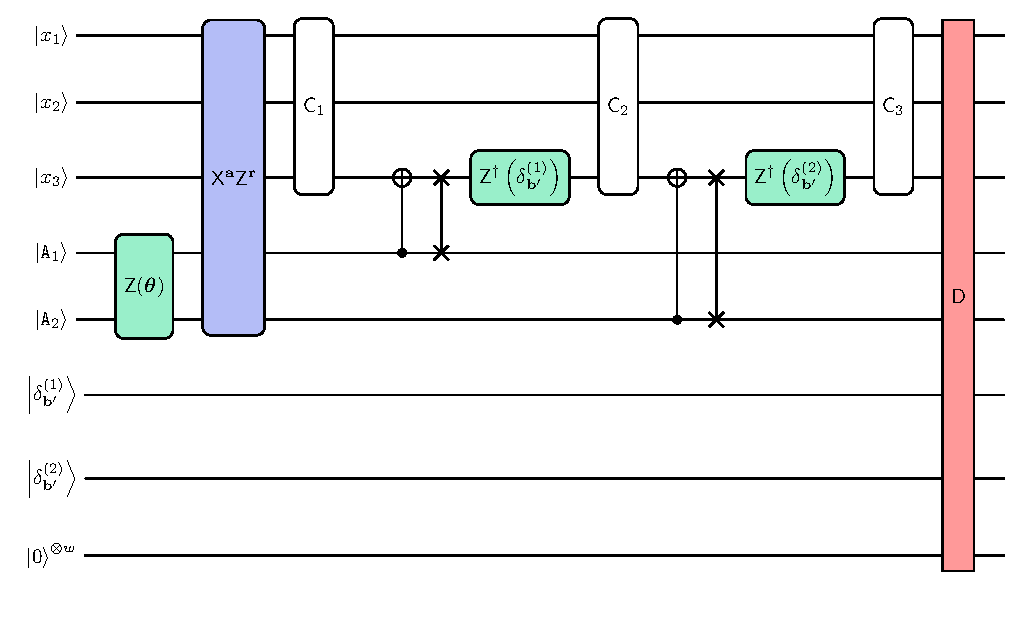
\includegraphics[width=\linewidth]{tikz-figures/blindness-proof/encryption-before.pdf}
        \caption{Representation of the state after interaction with a malicious Server, alongside the computation branch $\b'$, on a computation where $n=3, t=2$. The $\ketbra{\b'}{\b}$ operation is to be applied on the output wires.
        The protocol was unitarized and any malicious behavior can be written as a unitary operator $\D$ (red box) performed by the Server after executing the protocol honestly.
        This unitarization has transformed the classically-controlled rotations of Equation~\ref{eq:unitarization:avant} into simple $\Z^\dagger(\delta)$ rotations (green boxes in the circuit and see Equation~\ref{eq:unitarization:fin}) while the deviation is applied on the angles sent by the Client at the end of the honest execution.
        In this figure, the Client has sent the input and the ancillas $\rho\otimes \rho_{\A_1}\otimes... \otimes \rho_{\A_t}$ encrypted with a Pauli operator (blue box) and a pre-rotation on the ancillas (green box on the left), which later gets compensated during the $\Z^\dagger(\delta)$ rotations (green boxes in the middle).}
        \label{fig:mb-DQC-secproof-before commutation}
    \end{figure}

    \paragraph{Commuting the encryption.}
    The next step is to commute the initial Pauli encryption through the honest, unitary sequence of Clifford and state-injection layers. Similarly, as in the proof of correctness of Protocol~\ref{protocol:blind-gate}, after each layer the Pauli encryption is mapped to another Pauli encryption (a bijective mapping since the operations are Clifford). Also, the $\Z(\theta)$ pre-rotation can be commuted and gets cancelled in the $\Z(\delta_{\b'})$ rotation that becomes $\Z(\phi_{\b'})$, \emph{i.e.}, the correct rotation alongside branch $\b'$. This can be applied to all layers successively: the state of the total system before deviation remains encrypted.
    If we write the final encryption keys as $\a', \r'$ that, given $\b'$, are a deterministic Clifford mapping from $\a, \r$, the result can be depicted on Figure~\ref{fig:mb-DQC-secproof-after commutation}, and the state can be written as
    \begin{equation}
        \rho_{out, \b'}^{\a, \r, \boldsymbol{\theta}}
        =
        \ketbra{\b'}{\b}
        \circ
        \D
        \circ \Enc{\a'}{\r'}
        \left[
            \rho_{cor, \b', C}
            \otimes
            \ketbra{\boldsymbol\delta_{b'}}
            \otimes
            \ketbra{0}^{\otimes w}
        \right]
    \end{equation}
    where
         $\rho_{cor, \b, C} =
        \C_{t+1}
        \circ
        \Z^\dagger_n(\phi^{(t)}_{\b})
                \circ \F_{t}
                \circ \C_{t}
            \circ
            \cdots
            \circ
            \Z^\dagger_n(\phi^{(1)}_{\b})
                \circ \F_{1}
                \circ \C_{1}
        [\rho\otimes \rho_\A]
        $ is the correct state after honest Clifford and state injection layers for computation $C$ alongside computation branch $\b$ (used for branch $\b'$ in the above, since the Client stores $\b'$).

            \begin{figure}[h]
        \centering
        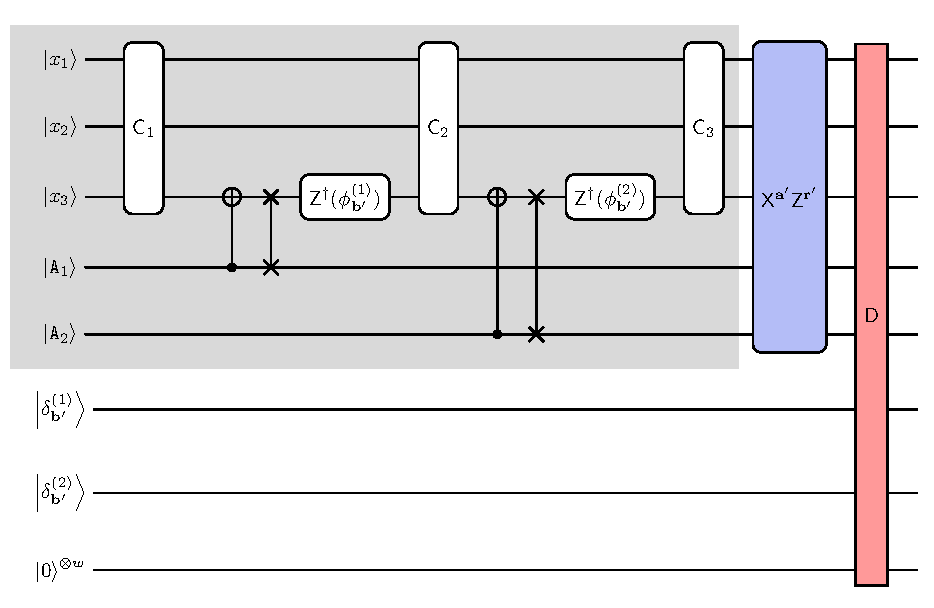
\includegraphics[width=\linewidth]{tikz-figures/blindness-proof/encryption-after.pdf}
        \caption{Same as Figure~\ref{fig:mb-DQC-secproof-before commutation}, but with a commuted encryption. On each layer, the $\Z({\theta})$ encryption is absorbed into $\Z^\dagger(\delta)$ to turn it into $\Z(\phi)$, so the green boxes of Figure~\ref{fig:mb-DQC-secproof-before commutation} disappear. The Pauli encryption $\Enc{\a}{\r}$ is commuted through the entire Clifford circuit and results in $\Enc{\a'}{\r'}$ (blue box in the figure). The state in the gray box is $\rho_{cor, \b', C}$, \emph{i.e.}, the correct state after honest execution of the protocol alongside branch $\b'$.}
        \label{fig:mb-DQC-secproof-after commutation}
    \end{figure}

    Then, we show that decoding measurement outcomes can be seen as applying a decryption operator before the measurements, and that is the conjugate of the encryption operator. This is straightforward: the Client's decoding corresponds to storing $\b'=\b\oplus \a'$, since indeed at each step, the Client decrypts the measurement outcomes with the $\X$-factor of the encryption. On the level of the entire computation, it amounts to storing $\b$ as $\b'=\b\oplus \a'$. Hence, it is equivalent to applying a decryption $\X^{\a'}$ before the $\Z$-basis measurement, which is equivalent to a $\Dec{\a'}{\r'}$ decryption since the measurement basis is invariant under $\Z$. Formally, let the following change of variables: $\b'' = \b\oplus \a'$, so that $\b$ becomes $\b''\oplus \a'$, and $\b'$ becomes $\b''$. Then, re-label $\b''$ as $\b$. We thus have:
        \begin{equation}
            \rho_{out, \b}^{\a, \r, \boldsymbol{\theta}}
            =
            \ketbra\b
            \circ
            \Dec{\a'}{\r'}
            \circ
            \D
            \circ
            \Enc{\a'}{\r'}
            \left[
                \rho_{cor, \b, C}
                \otimes
            \ketbra{\boldsymbol\delta_{b}}
            \otimes
            \ketbra{0}^{\otimes w}
            \right]
        \end{equation}

    \paragraph{From the point of view of the Distinguisher.}
    From the point of view of any unbounded Distinguisher, the keys $\a, \r$ are unknown, so the resulting state is a statistical mixture of all the possible values of $\a, \r$ over $\bin^{n+t}$ since they follow a uniform distribution. The updated keys $\a', \r'$ do as well since at each layer they are updated according to a Clifford transformation, which is a bijection. The result is that the sum can be similarly taken over $\a', \r'\in\bin^{n+t}$, which we re-label $\a, \r$ for simplicity. Furthermore, the angles $\theta_i$ for $i\leq t$ are not known neither, so a sum must be taken on the possible values of $\boldsymbol{\theta}$ over $\Theta^{t}$.
        We get:
        \begin{align}
            \rho_{out, \b}&=
            \dfrac{1}{4^{n+t}}
            \sum_{\a, \r\in \bin^{n+t}}
            \dfrac{1}{2^{2t}}
            \sum_{\boldsymbol{\theta}}
            \ketbra\b
            \circ
            \Dec{\a}{\r}
            \circ
            \D
            \circ
            \Enc{\a}{\r}
            \left[
                \rho_{cor, \b, C}
                \otimes
            \ketbra{\boldsymbol\delta_{b}}
            \otimes
            \ketbra{0}^{\otimes w}
            \right]
        \end{align}
        Now we notice that the values of $\theta$ only appears in the angles register. Since their distribution is uniform, they perfectly one-time pad that register and yield the maximally mixed state on $2$ qubits for each layer so $2t$ qubits in total, which can be discarded from the state since it contains no useful information. We organize the above sum to make that clear
        \begin{align}
            \rho_{out, \b}
            &=
            \dfrac{1}{4^{n+t}}
            \ketbra\b
            \left[
                \sum_{\a, \r\in \bin^{n+t}}
                \Dec{\a}{\r}
                \circ
                \D
                \circ
                \Enc{\a}{\r}
                \left[
                    \rho_{cor, \b, C}
                    \otimes
                \left( \dfrac{1}{2^{2t}}
                \sum_{\boldsymbol{\theta}}
                \ketbra{\boldsymbol\delta_{b}} \right)
                \otimes
                \ketbra{0}^{\otimes w}
                \right]
            \right]
            \\
            &=
            \dfrac{1}{4^{n+t}}
            \ketbra\b
            \left[
                \sum_{\a, \r\in \bin^{n+t}}
                \Dec{\a}{\r}
                \circ
                \D
                \circ
                \Enc{\a}{\r}
                \left[
                    \rho_{cor, \b, C}
                    \otimes
                \left( \dfrac{\id_{2t}}{2^{2t}}
                 \right)
                \otimes
                \ketbra{0}^{\otimes w}
                \right]
            \right]
            \\
            \label{eq:paulidev:beforePOV}
            &=
            \dfrac{1}{4^{n+t}}
            \ketbra\b
            \left[
                \sum_{\a, \r\in \bin^{n+t}}
                \Dec{\a}{\r}
                \circ
                \D
                \circ
                \Enc{\a}{\r}
                \left[
                    \rho_{cor, \b, C}
                \otimes
                \ketbra{0}^{\otimes w}
                \right]
            \right]
        \end{align}

        Without loss of generality, we can always decompose $\D$ in the $n+t$-qubit Pauli basis as $\D=\sum_{\E\in\Pauli_{n+t}}\alpha_\E \E\otimes \U_\E$ where $\E$ acts on the $n+t$-qubit system sent by the Client while $\U_\E$ acts on the rest of the system (meaning the working register, since the angle register has been traced out). This choice is convenient because it is on this $n+t$ qubit subsystem that the encryption and decryption occurs, and hence the Pauli Twirling lemma will apply. Indeed, the following simplification can now occur:
        \begin{align}
            \label{eq:twirl begin}
            &\dfrac{1}{4^{n+t}}\sum_{\a, \r\in\bin^{n+t}}
                \Dec{\a}{\r}
                \circ
                \D
                \circ
                \Enc{\a}{\r}
                \left[
                    \rho_{cor, \b, C}
                \otimes
                \ketbra{0}^{\otimes w}
                \right]
                \\
                &=
            \dfrac{1}{4^{n+t}}\sum_{\a, \r\in\bin^{n+t}}
                \Dec{\a}{\r}
                \circ
                \left(
                    \sum_{\E\in\Pauli_{n+t}}\alpha_\E \E\otimes \U_\E
                 \right)
                \circ
                \Enc{\a}{\r}
                \left[
                    \rho_{cor, \b, C}
                \otimes
                \ketbra{0}^{\otimes w}
                \right]
                \\
                &=
                \dfrac{1}{4^{n+t}}\sum_{\E, \E'\in \Pauli_{n+t}}
                \alpha_\E
                \alpha^*_{\E'}
                \sum_{\Q \in \Pauli_{n+t}}
                \Q^\dagger
                \E
                \Q
                \;
                \rho_{cor, b}
                \;
                \Q^\dagger
                \E^{\prime \dagger}
                \Q
                \otimes \U_{\E}\ketbra0^{\otimes w}\U^\dagger_{\E'}
                \\
                &=
                \dfrac{1}{4^{n+t}}\sum_{\E\in \Pauli_{n+t}}
                \abs*{\alpha_\E}^2
                \sum_{\Q \in \Pauli_{n+t}}
                \Q^\dagger
                \E
                \Q
                \;
                \rho_{cor, b}
                \;
                \Q^\dagger
                \E^{\dagger}
                \Q
                \otimes \U_{\E}\ketbra0^{\otimes w}\U^\dagger_{\E}
                \\
                \label{eq:twirl end}
                &=
                \dfrac{1}{4^{n+t}}\sum_{\E\in \Pauli_{n+t}}
                \abs*{\alpha_\E}^2
                \sum_{\Q \in \Pauli_{n+t}}
                \Q^\dagger
                \circ
                \E
                \circ
                \Q[\rho_{cor, b}]
                \otimes \U_\E[
                    \ketbra0^{\otimes w}
                ]
                \\
                \label{eq:encryption commute}
                &=
                \sum_{\E\in \Pauli_{n+t}}
                \abs*{\alpha_\E}^2
                \E
                [\rho_{cor, b}]
                \otimes \U_\E[
                    \ketbra0^{\otimes w}
                ]
        \end{align}
        where in Equations~\ref{eq:twirl begin} to~\ref{eq:twirl end} we simply applied the Pauli Twirl Lemma~\ref{lemma:Pauli Twirl}, and to obtain Equation~\ref{eq:encryption commute} we used the fact that Pauli operators commute up to an irrelevant global phase.
        Hence,
        \begin{equation}
            \rho_{out, \b} =
            \sum_{\E\in \Pauli_{n+t}}
            \abs*{\alpha_\E}^2
            \ketbra \b
            \circ
            \E
            [\rho_{cor, b}]
            \otimes \U_\E[
                \ketbra0^{\otimes w}
            ]
        \end{equation}

        Averaging over the all the computation branches yields the result stated in the initial lemma:
        \begin{align}
            \rho_{out}
        =
            \dfrac{1}{2^{n+t}}
            \sum_{\b\in\bin^{n+t}}
            \rho_{out, \b}
        \end{align}

\end{proof}
 \subsection{Security of Magic-Blind Delegated Quantum Computation}
\label{subsection:security proof MB-DQC}

\begin{proof}
    The security proof of Magic-Blind DQC in the Abstract Cryptography framework amounts to proving indistinguishability between the Real World and the Ideal World. In this proof, we analyze the transcript in the Real World, and present a Simulator that, once plugged into the Resource, allows one to generate the same transcript, concluding the proof. In what follows, let the inputs (computation and input state) chosen by the Distinguisher be $C$ and $\rho$.

    \paragraph{In the Real World.}
    We start with the transcript in the Real World. Here, we can use the work done in the proof of Lemma~\ref{lemma:mblind:Pauli deviations}, \textit{i.e.}, Section~\ref{subsection:proof of reduction to Pauli Dev}, which analyzes the evolution of the state when interacting with a malicious Server in Protocol~\ref{protocol:mblind_DQC}. Namely, after averaging over the possible secrets, using Equation~\ref{eq:paulidev:beforePOV} we can write the transcript in the Real World as
    \begin{equation}
        \rho_{real, out, \b}
        =
        \dfrac{1}{4^{n+t}}
            \ketbra\b
            \left[
                \sum_{\a, \r\in \bin^{n+t}}
                \Dec{\a}{\r}
                \circ
                \D
                \circ
                \Enc{\a}{\r}
                \left[
                    \rho_{cor, \b, C}
                \otimes
                \ketbra{0}^{\otimes w}
                \right]
            \right]\; .
    \end{equation}

    \paragraph{In the Ideal World.}
    We now present a Simulator that interacts with the malicious Server and Resource~\ref{resource:mblind_DQC}, and prove that it generates the same transcript as in the Real World. To do so, we proceed by reduction, as in the security proof of the Blind State Injection Protocol~\ref{protocol:blind-gate}. We present Reduction~\ref{reduction:MB-DQC}, show that it generates the same transcript as Protocol~\ref{protocol:mblind_DQC} (namely $\rho_{real, out, \b}$ for the same computation branch $\b$), and finally present a version using the Simulator and the Resource that performs the same steps and therefore generates the same transcript.

    \subparagraph{Presenting the Reduction.}
    To obtain Reduction~\ref{reduction:MB-DQC}, we replace the initial $n$-qubit encryption by an EPR encryption, and each "Clifford + Blind state injection" layer by its EPR-reduction version with delayed rotations, as already presented and analyzed in Reduction~\ref{protocol:blind-gate-reduction}. Finally, the Client receives $n$ bits from the Server and decodes them in the same way as in the initial protocol.

    \begin{reduction}
    \caption{MB-DQC, EPR-reduction and delayed rotations}
    \label{reduction:MB-DQC}
    \begin{algorithmic}[1]
        \Procedure{Client — EPR-encryption of $\rho$}{}
        \State Prepare $n$ EPR Pairs, and send each half to the Server.
        \State Perform Bell measurements on the other halves and $\rho$, set the $n$-bit outcome strings $\a, \r$ as encryption keys on $n$ bits.
        \EndProcedure

        \Procedure{Client — Perform Clifford and Injection layers}{}

        \For{$i=1, ..., t$}
        \State Prepare an EPR pair and send half to the Server.
        \State EPR-encrypt ancilla $\rho_{\A_i}$, part $1$, get outcome $x_i$.
        \State Set $\a'\gets \a||x_i, \r'\gets \r||0$
        \State Set $\a', \r'\gets \F_i\circ\C_{i}(\a', \r')$
        \State Receive bit $b_i$ from the Server.
        \State Decode $b_i \gets b_i \oplus a'_{n+i}$
        \State Sample $\delta_i \gets \$\Theta$ and sends it to the Server.
        \State Compute $\phi_i(\A_i, b_i)$ according to Equation~\ref{eq:blind:phi}
        \State Compute $\theta_i(\phi_i, a'_n, \delta_i)$ according to Equation~\ref{eq:blinded angle inverted}
        \State EPR-Encrypt ancilla $\rho_{\A_i}$, part $2$, pre-rotation angle $\theta$, get outcome $z_i$
        \State Set $\a\gets\a||x_i, \r\gets \r||z_i$, and re-update $\a', \r'\gets \F_i\circ \C_i(\a, \r)$
        \State Update $a'_n \gets a'_n\oplus b_i$ if $\A_i=\Tlabel$

        \EndFor
        \EndProcedure

        \Procedure{Client — Blind measurements}{}
        \State Truncate $\a, \r$ to the first $n$ bits.
        \State Receive $n$-bit string $\z$ from the Server.
        \State Update $\a, \r\gets \C_{t+1}(\a, \r)$
        \State Decode $\z\gets \z\oplus \a$
        \EndProcedure

        \State Output $\z$ as Client output if $\star$ ; else $\b||\z$.
    \end{algorithmic}
    \end{reduction}

    \subparagraph{Transcript in Reduction~\ref{reduction:MB-DQC}.}
To write the transcript that is generated when a Distinguisher interacts with Reduction~\ref{reduction:MB-DQC} instead of Protocol~\ref{protocol:mblind_DQC}, we proceed with the same logic as the proof of Lemma~\ref{lemma:mblind:Pauli deviations} in Section~\ref{subsection:proof of reduction to Pauli Dev}. We start by writing the state sent to the Server, by fixing the randomness—which here consists of the outcomes of the Bell measurements $\a, \r$ and the angle sampled uniformly by the Client $\boldsymbol\delta$—and the computation branch $\b$. We can note the following: after the EPR-encryption of $\rho$, the Bell measurement outcomes are $n$-bit strings $\a, \r$ and the Server holds $\Enc{\a}{\r}[\rho]$.

    Fixing the randomness $\boldsymbol{\delta}$ fixes the angles register to $\ketbra{\boldsymbol{\delta}}$. Then, fixing the computation branch $\b$ fixes for each $i\leq t$ the angle $\theta_i$. Using the same reasoning as for Reduction~\ref{protocol:blind-gate-reduction}, the qubit that the Server receives for each layer is in state $\Enc{x_i}{z_i}\circ\Z(\theta_i)[\rho_{\A_i}]$ after the Client's operations (EPR-encryption part $1$ and later $2$).
    Note that at each layer, one qubit is added so there is one more bit to the encryption keys: at the end $\a$ and $\r$ are $n+t$-bit encryption keys.
    Thus, without loss of generality, we can write that from the point of view of the Client that knows the outcomes $\a, \r$ and random angle $\boldsymbol{\delta}$, the qubits that are sent to the Server are, after the Client's operations, in the state
    \begin{equation}
        \rho_{red, in, \b}^{\a, \r, \boldsymbol{\delta}}
        =
        \Enc{\a}{\r}
            \circ
            \Z(\boldsymbol\theta)
            \left[\rho
            \otimes
            \rho_\A
            \otimes
            \ketbra{\boldsymbol\delta}
            \otimes
            \ketbra{0}^{\otimes w}\right]\; .
    \end{equation}

    The interaction with the malicious Server can be analyzed the same way as in the Real World. See Section~\ref{subsection:proof of reduction to Pauli Dev} for more details. Hence, after interaction, the state is
    \begin{equation}
            \rho_{red, out, \b}^{\a, \r, \boldsymbol{\delta}}
            =
            \ketbra\b
            \circ
            \Dec{\a'}{\r'}
            \circ
            \D
            \circ
            \Enc{\a'}{\r'}
            \left[
                \rho_{cor, \b, C}
                \otimes
            \ketbra{\boldsymbol\delta}
            \otimes
            \ketbra{0}^{\otimes w}
            \right]\; .
        \end{equation}
        From the point of view of the Distinguisher, the secrets $\a, \r, \boldsymbol{\delta}$ are unknown so we average over all the possible secret values (see Section~\ref{subsection:proof of reduction to Pauli Dev} for more details). Again, we clearly see that since $\boldsymbol{\delta}$ only appears in the angle register, it implements a one-time pad on $2t$ qubits and can safely be discarded. Thus,
            \begin{equation}
        \rho_{red, out, \b}
        =
        \dfrac{1}{4^{n+t}}
            \ketbra\b
            \left[
                \sum_{\a, \r\in \bin^{n+t}}
                \Dec{\a}{\r}
                \circ
                \D
                \circ
                \Enc{\a}{\r}
                \left[
                    \rho_{cor, \b, C}
                \otimes
                \ketbra{0}^{\otimes w}
                \right]
            \right]
            \; .
    \end{equation}
    We thus have $\rho_{red, out, \b} = \rho_{real, out, \b}$.

    \paragraph{Introducing the Simulator and concluding the proof.}
    We now present Simulator~\ref{simulator:MB-DQC}: in total, the operations performed by the Simulator and the Resource (via the CPTP map instructed by the Simulator) are the same as in Reduction~\ref{reduction:MB-DQC}

    \begin{simulatorr}
    \caption{MB-DQC}
    \label{simulator:MB-DQC}
    \begin{algorithmic}[1]
        \Procedure{Simulator - Emulates Client interaction with Server}{}
        \State Prepare $n$ EPR Pairs, and send each half to the Server.
        \For{$i=1, ..., t$}
        \State Prepare an EPR pair and send half to the Server.
        \State Receive bit $b_i$ from the Server.
        \State Sample $\delta_i \gets \$\Theta$ and send it to the Server.
        \EndFor
        \State Receive $n$-bit string $\z$ from the Server.
        \EndProcedure

        \Procedure{Simulator - Make Resource reproduce the Server behavior}{}
        \State Send the remaining $n+t$ EPR halves, the $n+t$-bit string $\b||\z$, and the angles $\boldsymbol\delta=(\delta_1, ..., \delta_t)$ to Ideal Resource
        \State Send the below instructions as a CPTP map to the Resource to perform.
        \EndProcedure

        \State \textbf{Resource Inputs:} $\C_1, ..., \C_{t+1}$ (public info.), $\rho$ and $\A_1, ..., \A_t$ from the Client, and $n+t$ EPR-halves, $\b||\z, \boldsymbol{\delta}$ from the Simulator.
        \Procedure{Resource - EPR-encryption of $\rho$}{}
        \State Perform Bell measurements on the received EPR pairs and $\rho$, and set the $n$-bit strings $\a, \r$ of measurement outcomes as encryption keys.
        \EndProcedure

        \Procedure{Resource - Perform Clifford and Injection layers}{}
        \For{$i=1, ..., t$}
        \State EPR-Encrypt ancilla $\rho_{\A_i}$, part $1$, get outcome $x_i$.
        \State Set $\a'\gets \a||x_i, \r'\gets \r||0$
        \State Set $\a', \r'\gets \F_i\circ\C_{i}(\a', \r')$
        \State Decode $b_i \gets b_i \oplus a'_{n+i}$
        \State Compute $\phi_i(\A_i, b_i)$ according to Equation~\ref{eq:blind:phi}
        \State Compute $\theta_i(\phi_i, a'_n, \delta_i)$ according to Equation~\ref{eq:blinded angle inverted}
        \State EPR-Encrypt ancilla $\rho_{\A_i}$, part $2$, pre-rotation angle $\theta$, get outcome $z_i$
        \State Set $\a\gets\a||x_i, \r\gets \r||z_i$, and re-update $\a', \r'\gets \F_i\circ \C_i(\a, \r)$
        \State Update $a'_n \gets a'_n\oplus b_i$ if $\A_i=\Tlabel$
        \EndFor
        \EndProcedure

        \Procedure{Resource - Perform Blind Measurements}{}
        \State Truncate $\a, \r$ to the first $n$ bits.
        \State Update $\a, \r\gets \C_{t+1}(\a, \r)$
        \State Decode $\z\gets \z\oplus \a$
        \EndProcedure

        \State Output $\z$ as Client output if $\star$ ; else $\b||\z$.
    \end{algorithmic}
    \end{simulatorr}

    Therefore, for the same randomness we have $\rho_{red, out, \b}^{\a, \r, \boldsymbol{\delta}} = \rho_{ideal, out, \b}^{\a, \r, \boldsymbol{\delta}}$, where $\rho_{ideal, out, \b}^{\a, \r, \boldsymbol{\delta}}$ is the transcript in the Ideal World.
    Hence, using the same reasoning, we conclude that $\rho_{ideal, out, \b} = \rho_{real, out, \b}$, and thus the protocol is perfectly secure.

\end{proof}
